\chapter{Field Applications}

\todo[inline]{This section will be integrated into the Experimental Platform}

\begin{wrapfigure}{l}{7cm}
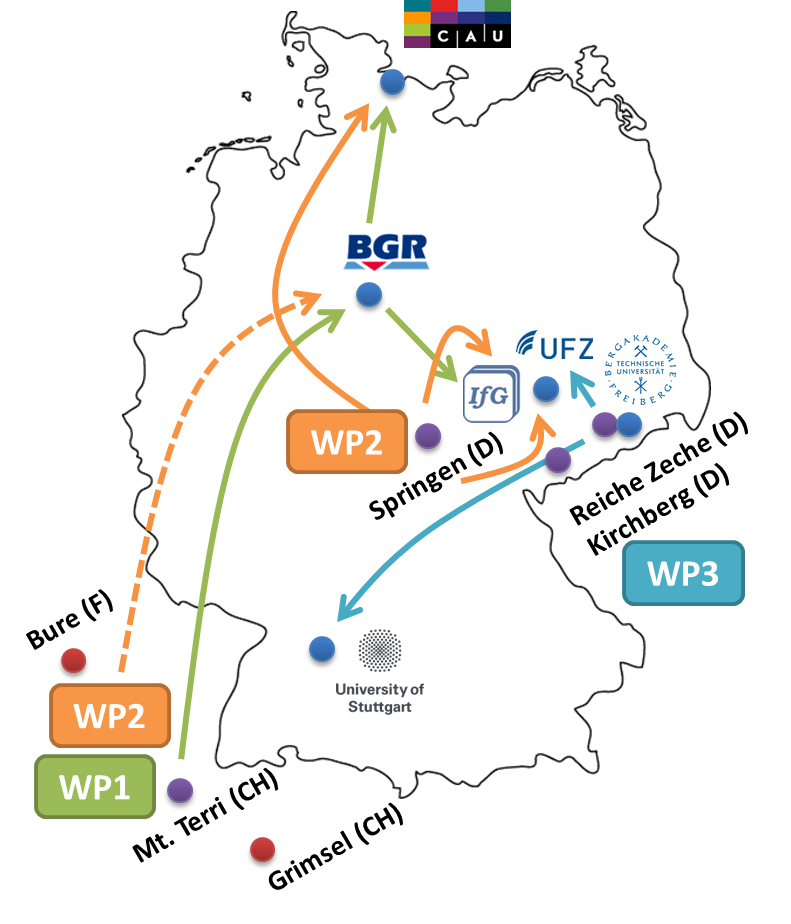
\includegraphics[width=6.9cm]{figures/geomint-exp.png}
\caption{Field sites for GeomInt}
\label{fig:geomint-sites}
\end{wrapfigure}
The GeomInt project is closely linked to the Underground Research Laboratory in Mont Terri (Switzerland) as well as to the German sites Springen (Thuringia) and Kirchberg/Freiberg (Saxony) not only in order to get specimen for experimental work, i.e. Opalinus clay, salt and crystalline rock samples, respectively, but also for being involved into in-situ experimental and real scale modeling works.
Fig. \ref{fig:geomint-sites} depicts the location of the sites as well as the geographic workflow of the sample material. BGR is providing Opalinus clay samples from the URL Mt. Terri for WP1 and WP2. Salt specimen for WP2 are offered by IfG, and crystalline rock material is delivered by TUBAF from the Kirchberg mine as well as the URL ''Reiche Zeche'' in Freiberg.

\begin{figure}
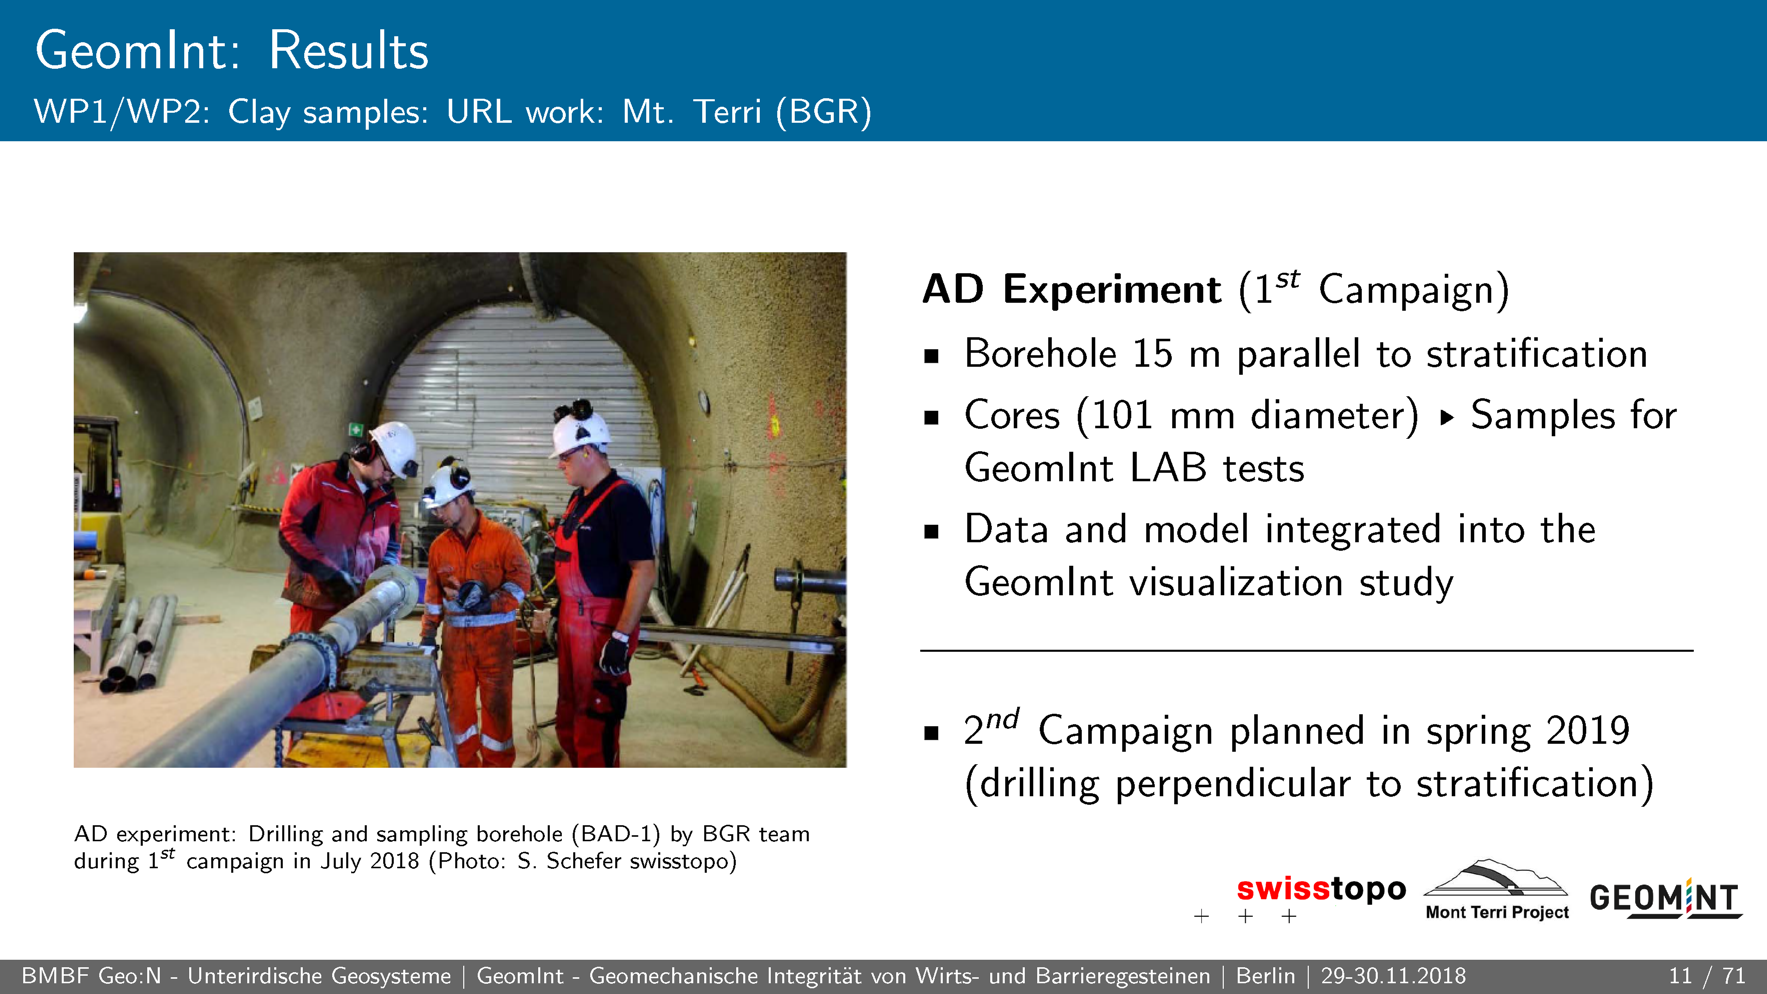
\includegraphics[width=0.9\textwidth]{figures/geomint-mt-terri.png}
\caption{URL Mt. Terri}
\label{fig:geomint-exp}
\end{figure}

\section{Kirchberg mine and URL ''Reiche Zeche''}

\begin{list}{-}{\leftmargin=1em \itemindent=0em \itemsep=0.2em}
\item ...
\end{list}
